\documentclass[12pt,a4paper]{article}
\usepackage[german]{babel}
\usepackage[T1]{fontenc}
\usepackage[utf8x]{inputenc}
\usepackage{url}
\usepackage{graphicx}
\usepackage{algpseudocode}
\usepackage{algorithm}
\usepackage{geometry}
\usepackage{amsfonts}
\usepackage{amsmath}
\usepackage{tabularx}
\usepackage{txfonts} %Times New Roman Font
\usepackage{titlesec} %Format der Headings ändern
\usepackage{hyperref}
\usepackage{comment}
\usepackage{listings}
\usepackage{pythonhighlight}

\renewcommand{\thesection}{\arabic{section}.} %Nummerierung der Sections anpassen
\renewcommand{\labelenumi}{\alph{enumi})}  %Nummerierung der Listen anpassen
%\titleformat{\section}{\large\bfseries}{\thesection}{0.5em}{} %Format der Section Überschrift ändern
\setlength{\parindent}{0pt} %Keine Einrückung bei neuen Paragraphen
\geometry{left=2.0cm,textwidth=17cm,top=2.5cm,textheight=23cm}

% Anpassen %
%%%%%%%%%%%%%%%%%%%%%%%%%%%%%%%%%%%%%
\newcommand{\student}{Daniel Pantjuskin-Moos\\ 108013248222 } % Namen eintragen
\newcommand{\partner}{Vincent König\\ 108011232630} % Matrikelnummer eintragen
\newcommand{\group}{D} % Gruppennummer eintragen
%%%%%%%%%%%%%%%%%%%%%%%%%%%%%%%%%%%%%

\newcommand{\hwheadtwo}{$ $
  \vspace{-2cm}
  
\noindent \student \qquad \qquad  Wireless Physical Layer Security Praktikum \hfill SS 2020 \\
\noindent \partner \\
%\noindent \thirdone \\  % einkommentieren, falls ihr eine 3er Gruppe seid
\noindent Gruppe:~\group\\
$ $

  
\begin{center}    
{\Large \bf Abgabe PHYSEC 5}
\end{center}
}

\begin{document}
\hwheadtwo

\renewcommand{\thesection}{\arabic{section}}
\section{Implementierung, Analyse, Theorie}


Der \textit{Sourcecode} und die dazugehörigen \textit{Plots} können	
\href{https://mega.nz/file/Tp5BXTJT#VjmofQ7s2OlpbuZjRIcCgFyBOkAGJOaEPOxHiNdmeKU}
{hier}
heruntergeladen werden.

\subsection{Analyse I}


\begin{itemize}
    \item Vergleichen Sie das obige Messsetup mit dem von 
    Ihnen verwendeten Setup während des
    Praktikums und setzen Sie die mögliche Menge an 
    extrahierbaren Bits in Vergleich zu den
    RSSI-Werten
\end{itemize}

Da im jetzigen Assignment 5 mit CSI-Daten gearbeitet wird,
ist die zu verarbeitende Menge an Daten wesentlich größer.

\begin{itemize}
    \item Überlegen Sie, welchen Vorteil RSSI-Werte 
    gegenüber den komplexen Kanalimpulsantworten
    haben
\end{itemize}

RSSI-Werte sind einfacher zu verarbeiten, da sie weniger 
Rechenaufwand nach sich ziehen und weniger Speicherplatz 
benötigen. Außerdem ist die Programmierarbeit einfacher 
für RSSI-Werte.


\newpage
\subsection{Theorie}

Hierbei wurde sich unter anderem auf dieses 
\href{https://ieeexplore.ieee.org/stamp/stamp.jsp?tp=&arnumber=6823677} 
{Paper (Seite 1132)} 
und diese 
\href{https://limo.libis.be/primo-explore/fulldisplay?docid=LIRIAS1662210&context%=L&vid=Lirias&search_scope=Lirias&tab=default_tab&lang=en_US&fromSitemap=1}
{Doktorarbeit (Seite 20 ff.)}
gestützt, welche kostenlos downloadbar sind.

\subsubsection*{Intradistanz}
\begin{comment}
VL 5, Folie 36:
Distance between responses for the same challenges. 
Shows measurements error


Doktorarbeit, S.20:
A PUF response intra-distance is a random variable
describing the distance between two PUF responses 
from the same PUF instance and using
the same challenge

Paper, S. 1132:
Intra-PUF variation: Defined as the number of bits
in a PUF response that vary when an identical
challenge is repeatedly queried on a given PUF
device in a changing environment. This variation is
due to this environmental change as well as 
statistical noise. As a result, it is commonly 
represented in the form of a statistical 
distribution. Intra-PUF variation is a measure of 
the reproducibility of responses from an individual 
PUF circuit.
\end{comment}

Beschreibt die Distanz zwischen den
\textit{Responses} für die selbe \textit{Challenge}. 
Man kann es als Indikator für die Größe des Messfehlers,
als auch laut dem Paper als Messwert für die 
Reproduzierbarkeit betrachten. Die Unterschiede entstehen 
durch Umwelteinflüsse und \textit{statistical Noise}.\\

In der Praxis kann dieser Wert, ähnlich wie in 
den Kommentaren zu \verb|compute_intra_distance| 
von Aufgabe 1.3 beschrieben, berechnet werden: Die
erste Messung einer \textit{Challenge} wird als Referenz 
genommen. Anschließend wird der euklidsche Abstand zu 
allen Messungen der selben \textit{Challenge} berechnet.
Das wird für alle \textit{Challenges} wiederholt.


\subsubsection*{Interdistanz}
\begin{comment}
VL 5, Folie 36:
Distance between responses for different challenges. 
Indicates uniqueness of responses.

Doktorarbeit, S. 22:
A PUF response inter-distance is a random variable 
describing the distance between two PUF responses 
from different PUF instances using the same challenge:


Paper, S. 1132:
Inter-PUF variation: Defined as the number of bits
in a PUF response that vary between different
devices for a set of shared challenges. This is 
due to differences between the physical ICs and 
is also commonly represented in the form of a 
statistical distribution. The inter-PUF variation 
is a measure of the uniqueness of an individual 
PUF circuit
\end{comment}

Distanz zwischen \textit{Responses} für verschiedene 
\textit{Challenges} und laut dem Paper ein Indikator 
für die Einzigartigkeit eines \textit{PUF circuit}
beziehungsweise laut Vorlesung 5, Folie 36 ein Indikator
für die Einzigartigkeit der \textit{responses}.\\ 


In der Praxis, kann es ähnlich wie in der Aufgabe 1.3 
bei der Funktion \verb|compute_inter_distance| 
aussehen, wobei man hier die Anzahl der
zu berechnenden Distanzen gering halten möchte.
Deswegen beschränkt man sich auf die jeweils ersten 
Messungen jeder \textit{Challenge}: Dazu werden alle 
Distanzen aller Paare, ungeordnet und ohne Zurücklegen, 
gebildet von den ersten Messungen aller 
\textit{Challenges}, was somit 
\footnotesize $\binom{40}{2}=780$ \normalsize
verschiedene Paare sind. 


\newpage
\subsection{Implementierung}
Test
\newpage
\subsection{Analyse II}
Test
\newpage
\section{Implementierung Quantisierer}

Hier Aufgabe 2 bearbeiten
\subsection{Implementierung Jana Multibit}

\subsection{Implementierung Mathur, Suhas}

\begin{comment}
% Beispiel für einen Hyperlink 	
\href{https://www.rub.de}{hier klicken}

% Beispiel für Bilder mit Caption und Referenz
\begin{figure}[hbt!]
	\centering
		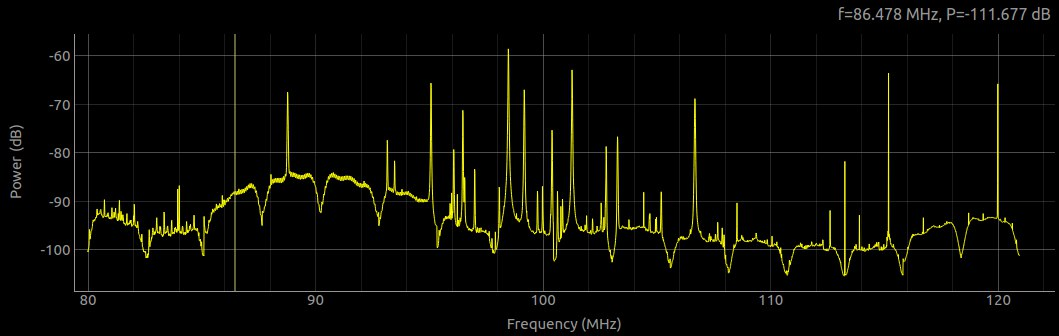
\includegraphics[width=1\textwidth]
		{Bilder/a3_rtl_sdr.jpg}
		\caption{Hier Caption einfügen}
		\label{fig:Labelx}
\end{figure}

% Als Beispiel wie man referenziert
~\ref{fig:Labelx}

% Beispiel für das Einfügen von Python Code
\begin{python}
print("Hello World")
\end{python}

% Beispiel für das Erzwingen von Abstand (selbe Zeile)
\hspace{0.5mm}

% Beispiel für das Erzwingen von Abstand (nach unten)
\\[0.7cm]

%Beispiel für einen Pseudocode
\subsection*{b) Pseudocode}
\begin{algorithm}
\caption{Pseudocode}
\begin{algorithmic}[1]
\State $range = max[RSS] - min[RSS]$
\State $N \in [0, log_2 RSS]$
\State $M = 2^N$
\State $RSS[] \to M$ intervalls $I[]$ of equal size
\State Choose $N$ bit assignment $\forall$ $M$ intervalls
\For{$t \to len(RSS[])$}
\For{$i \to len(I[]$}
\If{$RSS[t] \in I[i]$}
\State $bitstream \gets$ bit assignment
\EndIf
\EndFor
\EndFor\\
\Return $bitstream$
\end{algorithmic}
\end{algorithm}

% Beispiel für ein Tabelle mit vergrößerter Schrift
\Large
\begin{tabular}{ |p{3cm}|||p{3cm}|p{3cm}||p{3cm}|p{3cm}|}
    \hline
    \multicolumn{5}{|c|}{Teilaufgabe 1: $A\rightarrow B$} \\
    \hline
    Blockgröße & Mittel Bob & Median Bob & Mittel Eve & Median Eve\\
    \hline
    \hspace{3.2mm}30 & 0.2290 & 0.1756 & 0.1798 & 0.1428\\
    100 & 0.2219 & 0.1848 & 0.1341 & 0.1053\\
    200 & 0.2401 & 0.2377 & 0.0946 & 0.0748\\
    250 & 0.2591 & 0.2328 & 0.1495 & 0.1260\\
    300 & 0.2791 & 0.2108 & 0.1784 & 0.1130\\
    \hline
\end{tabular}
\normalsize

% Öffnende und schließende deutsche Anführungszeichen
\glqq Zitierter Text komm hierhin \grqq  

% Kaligraphische Buchstaben im mathematischen Stil (ua) für
% Mengen verwendet. Hier G 
\( \mathcal{G} \)

% Ein Ausdruck hier compute_intra_distance in 
Code-Style-Ausgabe bzw. Arial-font (?)
\verb|compute_intra_distance|

% Leere neue Zeile erzwingen, 
% falls \newline nicht funktioniert
\hfill \break
\end{comment}

\end{document}